\documentclass[a4paper]{article}
\usepackage{graphicx}
\usepackage[english,russian]{babel}
\usepackage[utf8]{inputenc}
\usepackage[T2A]{fontenc}
\usepackage{tabto}
\usepackage{amsmath}
\usepackage{pgfplots}
\usepackage[left=25mm, top=20mm, right=10mm, bottom=10mm, nohead, nofoot]{geometry}
\usepackage{graphicx}
\DeclareGraphicsExtensions{.pdf,.png,.jpg}
\begin{document}
    \begin{center} 
        \LARGE Подготовка к зачету.\\
    \end{center}
    \newpage
    \section{Практика}
    1)Построить линию $(x-1)^2+(y+2)^2=4$\\
    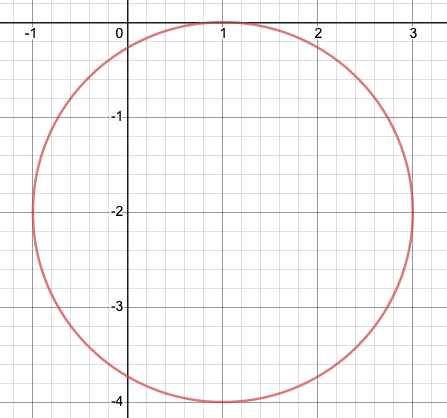
\includegraphics[scale=0.3]{e}\\
    2) Составить уравнение окружности с радиусом 7 с центром в точке C(2,-3)?\\
    $(x-2)^2+(y+3)^2=49$\\
    3)Построить линию $x=1-3sint,y=-2+3cost$
\end{document}